%\documentclass[10pt,krantz2]{krantz}
\documentclass[10pt]{book}
%\usepackage{sfheaders}        %% Chap/Sec headers in Helvetica;
\usepackage{graphicx}         %% well, its about graphics
\usepackage{blindtext}

\usepackage[paperwidth=7in,paperheight=10in]{geometry}

\usepackage{tikz}
\usetikzlibrary{mindmap,backgrounds}
\colorlet{col1}{teal}        %% Part I color
\colorlet{col2}{olive}       %% Part II
\colorlet{col3}{orange}      %% Part III

% local chapter commands
\newcommand{\chapterprelude}[1]{%
\textsf{#1}
\par\noindent
\rule{\textwidth}{0.4pt}
}
\newcommand{\hard}{$^\star$\xspace}

\setcounter{chapter}{2} % one less than chapter number

\usepackage{titlesec}

\newcommand{\chaptitle}[1]{%
\begin{tikzpicture}
  \node[fill=col1!20,inner sep=6pt,text width=\dimexpr\linewidth-12pt\relax] {#1};
\end{tikzpicture}
}

\titleformat{\chapter}[display]
{\normalfont\huge\bfseries\sffamily}{\scalebox{3}{\thechapter}}{25pt}{\Huge\chaptitle}
\titlespacing*{\chapter} {0pt}{110pt}{20pt}

\newsavebox{\mybox}


\begin{document}

\chapter{Fitting and Graphing Discrete Distributions}\label{ch:discrete}

%\input{ch03/vtoc}   %% visual contents images

\savebox\mybox{%
  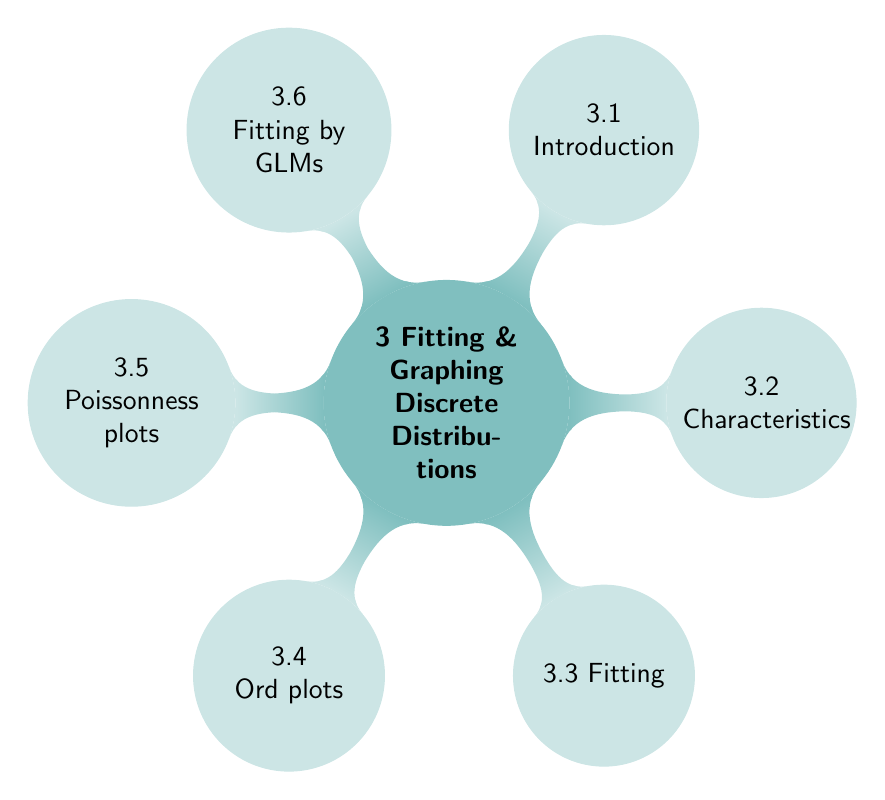
\begin{tikzpicture}[grow cyclic, text width=2cm, align=flush center,
                      every node/.style=concept, concept color=col1!50,
    level 1/.style={level distance=4cm, sibling angle=60,         %% 360/# of sections
                         concept color=col1!20,font=\sffamily},
%       level 2/.style={level distance=4.5cm,sibling angle=45, concept color=col1!20}
    ]
    \node[font=\bfseries\sffamily]  {3 Fitting \& Graphing Discrete Distributions} [clockwise from=60]  % root node
            child { node {3.1 \\ Introduction}}
            child { node {3.2 \\ Characteristics}}
            child { node {3.3 Fitting}}
            child { node {3.4 \\ Ord plots}}
            child { node {3.5 \\ Poissonness plots}}
            child { node (sec36) {3.6 \\ Fitting by GLMs}}
            ;
    \end{tikzpicture}
}

\begin{tikzpicture}[remember picture,overlay]
  \node[anchor=north east] at (current page.north east) {\usebox{\mybox}};
\end{tikzpicture}

\chapterprelude{%
Discrete data often follow various theoretical probability models.
Graphic displays are used to visualize goodness of fit,
to diagnose an appropriate model, and determine the impact of
individual observations on estimated parameters.
}

\section{Introduction to discrete distributions}\label{sec:discrete-intro}
\blindtext
\section{Characteristics of  discrete distributions}\label{sec:discrete-distrib}
\section{Fitting discrete distributions}\label{sec:discrete-fit}
\section{Diagnosing discrete distributions: Ord plots}\label{sec:discrete-ord}
\section{Poissonness plots and generalized distribution plots}\label{sec:discrete-Poissonness}
\section{Fitting discrete distributions as generalized linear models\hard}\label{sec:fitglm}

\end{document}
